We describe how we evaluate our results.

\subsection{Post-processing}
We aim to evaluate convolutional networks as a single end-to-end segmentation model;
%component in an end-to-end segmentation task;
thus, we choose to use the produced heatmaps without any post-processing. However, adding post-processing to our best performing architecture will certainly improve results and remains as a viable future endeavor.% In any case, having a strong network to start with is needed to produce good results.

% Options:
% uncorrected threshold: Select a threshold, take that as segementation
% Cluster-extent correction: Delete thresholds that are under a number of pixels 
% or whose total probability is less than a desired number. Needs this number
% Threshold-free cluster enhancement (module 29 in introduction to fmri): Same as aove but withouth a cluster (?)
% Number of clusters per image: do threshold-free enhancement where the metric is to 
% leave only the most promising cluster
% Conditional random fields (CRF): Work quite well. Python implementation of CRF: https://pystruct.github.io/auto_examples/image_segmentation.html Here is another take: http://www.robots.ox.ac.uk/~szheng/CRFasRNN.html Any look fine.

\subsection{Segmentation}
We generate a segmentation by setting each pixel whose value was zero in the original mammogram to background (0), each non-background pixel whose logit is greater than a threshold to breast mass (255) and any remaining pixel to normal breast tissue (127) (Fig.~\ref{fig:Post-processing}).

\begin{figure}[h]
	\centering
	\begin{subfigure}{0.2\textwidth}
		\centering
                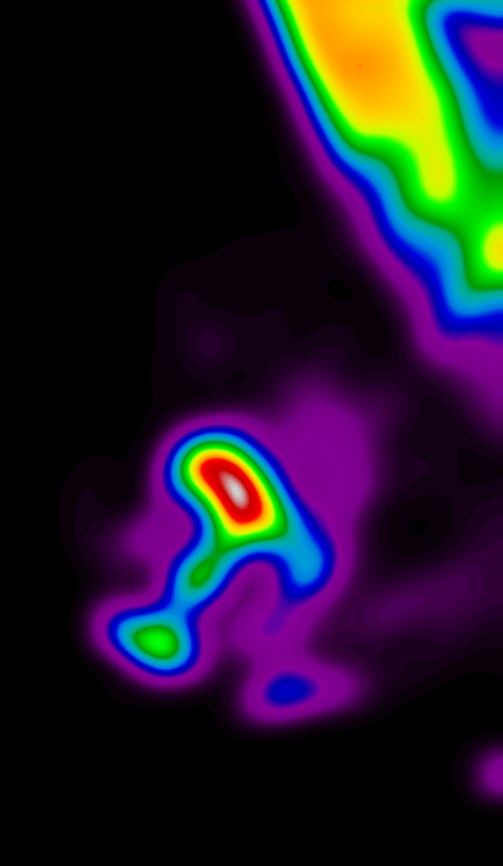
\includegraphics[width=\textwidth]{plots/probs.png}
         \caption{Prediction}
	\end{subfigure}
	\quad
	\begin{subfigure}{0.2\textwidth}
		\centering
                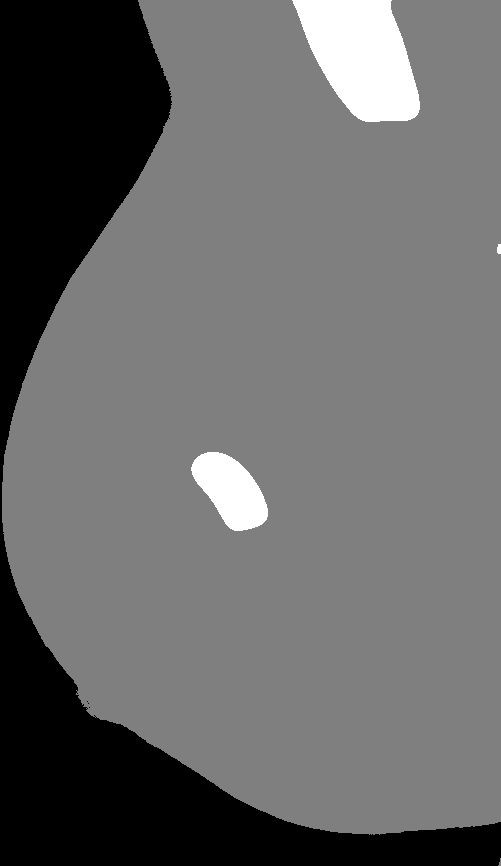
\includegraphics[width=\textwidth]{plots/segmentation.png}
         \caption{Segmentation}
	\end{subfigure}
	\caption[Post-processing pipeline]{Heatmap of probabilities and segmentation produced by assigning all background to black and thresholding at probability 0.5.}
	 \label{fig:Post-processing}
\end{figure}
% Using the validation set, we compute the IOU for different thresholds and select the one that produces the best result. The final segmentation is generated by setting each pixel whose value was zero in the original mammogram to background (0), each non-background pixel whose logit is greater than the threshold to breast mass (255) and any remaining pixel to normal breast tissue (127).

\subsection{Metrics}
We use five-fold cross-validation and the free-response ROC curve to evaluate our models. We count a breast mass as a true positive if a blob in the segmentation covers at least 10\% of its area. To avoid any bias, we compute the number of false positives per image only in the images without a breast mass~\cite{Chakraborty2013}. Furthermore, we force the number of false positives in an image to be non-decreasing for lower, i.e., laxer thresholds.
